%! TEX root = main.tex  %
\documentclass[main.tex]{subfiles} % Wichtig!

\begin{document}

\subsection{Projektmanagement}
Das Projektmanagement spielt eine zentrale Rolle in der Vorbereitungsphase meiner Bachelorarbeit 
und bildet die Grundlage für den Erfolg des gesamten Vorhabens. Dabei geht es nicht nur um die 
reine Planung, sondern auch um eine effiziente Steuerung und kontinuierliche Kontrolle aller 
Arbeitspakete und derer Ergebnisse. Die besondere Herausforderung meiner Arbeit liegt darin, 
das umfangreiche Themengebiet, das für diese Bachelorarbeit relevant ist, innerhalb des engen 
Zeitrahmens von 14 Wochen sinnvoll und fundiert zu bearbeiten. Das Themengebiet umfasst diverse 
Bereiche der Informatik. Darunter fallen Audioverarbeitung, maschinelles Lernen, 
Softwareentwicklung und auch einiges an mathematischem Hintergrundwissen. Daher wurde ein agiles 
Vorgehensmodell gewählt. Dies bedeutet, dass sowohl die Planung als auch die Umsetzung in iterative 
Zyklen unterteilt sind. Während es zu Beginn eine grobe Struktur und Zielsetzung gibt, ermöglicht 
diese Herangehensweise Flexibilität in der Durchführung. Dadurch können Veränderungen oder 
unerwartete Ereignisse leichter integriert und die Bachelorarbeit fortlaufend optimiert werden.

\subsubsection{Produkt Backlog}

Der Product Backlog beinhaltet alle Anforderungen die für dir Erstellung des 
Spracherkennungssystems. Die Erstellung des Models, die Entwicklung der 
mobile App und die Dokumentation sind dabei die Hauptaufgaben.



\begin{figure}[h]
    \centering
    
\includegraphics[width=0.4\linewidth]{img/placeholder.png}
    \caption{Tabelle für das anfängliche Product Backlog}
    \label{fig:backlog_table}
\end{figure}

\subsubsection{Risikomanagement}
Als mögliche Risiken wurden im Projekt zum einen die Komplexität des Themas und zum anderen die
begrenzte Zeit für die Bearbeitung identifiziert. Weitere Risiken, die während der 
Projektdurchführung aufgetreten sind, werden nachfolgend zusammengefasst. Die Tabelle 
\ref{tab:risiken} zeigt die identifizierten Risiken, deren Eintrittswahrscheinlichkeit sowie die 
Auswirkung auf das Projekt.

\begin{table}[h]
    \centering
    \begin{tabular}{|l|c|c|}
        \hline
        \textbf{Risiko} & \textbf{Eintrittswahrscheinlichkeit} & \textbf{Auswirkung} \\
        \hline
        Komplexität des Themas & Hoch & Gross \\
        \hline
        Begrenzte Zeit für Bearbeitung (14 Wochen) & Mittel & Kritisch \\
        \hline
        80\% Arbeitspensum, 20h pro Woche am Wochenende & Hoch & Mittel \\
        \hline
        Grosser Release in aktueller Arbeit bis Ende Oktober & Hoch & Hoch \\
        \hline
        Qualität des Speech Recognizers & Mittel & Kritisch \\
        \hline
        Latenz und Performance des Erkenners & Hoch & Gross \\
        \hline
    \end{tabular}
    \caption{Identifizierte Risiken im Projekt}
    \label{tab:risiken}
\end{table}



\begin{landscape}
    \subsection{Grobplanung}
    Die Grobplanung zeigt die wichtigsten Meilensteine sowie die anfängliche zeitliche Einteilung 
    der einzelnen Themenbereiche die für die Bachelorarbeit relevant sind, aufgezeigt. Die
    Grobplanung ist in Abbildung \ref{fig:grobplanung} dargestellt.

    \begin{figure}[!htb]
        \centering
        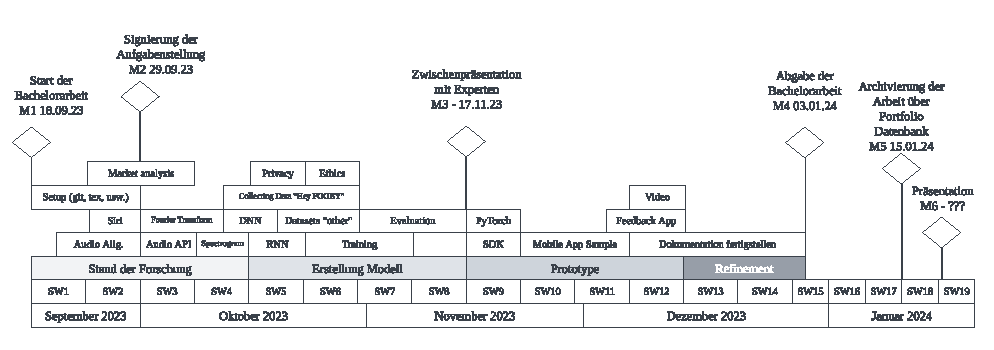
\includegraphics[width=\linewidth]{img/projectplan.pdf}
        \caption{Grobplanung}
        \label{fig:grobplanung}
    \end{figure}
\end{landscape}



\end{document}
